\section{Diagramas de atividades}
O detalhe de forma simples das ações do ator nos diferentes ecrãs foi realizado em diagramas de atividades.

\subsection{Diagrama de atividades página inicial}

Da página inicial da aplicação é possível deslocar para o fórum, para as notificações, para o perfil e realizar operações do catálogo.

\begin{figure}[htb]
    \centering
    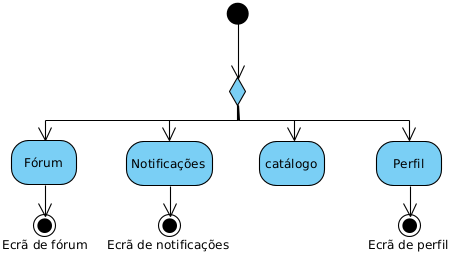
\includegraphics[width=0.6\textwidth]{images/diagramas/atividades/diagrama_atividades_home.png}
    \caption{Diagrama de atividades de página inicial da aplicação}
    \label{fig:34}
\end{figure}

\subsection{Diagrama de atividades página de perfil}

Na página de perfil, é possível alterar a imagem, o nome, o \textit{email}, selecionar os métodos e os tipos de notificação a receber. Caso uma empresa veja o perfil esta poderá, além das operações acima mencionadas, gerir os recursos humanos onde é encaminhada para o ecrã de gestão de recursos humanos.

\begin{figure}[htb]
    \centering
    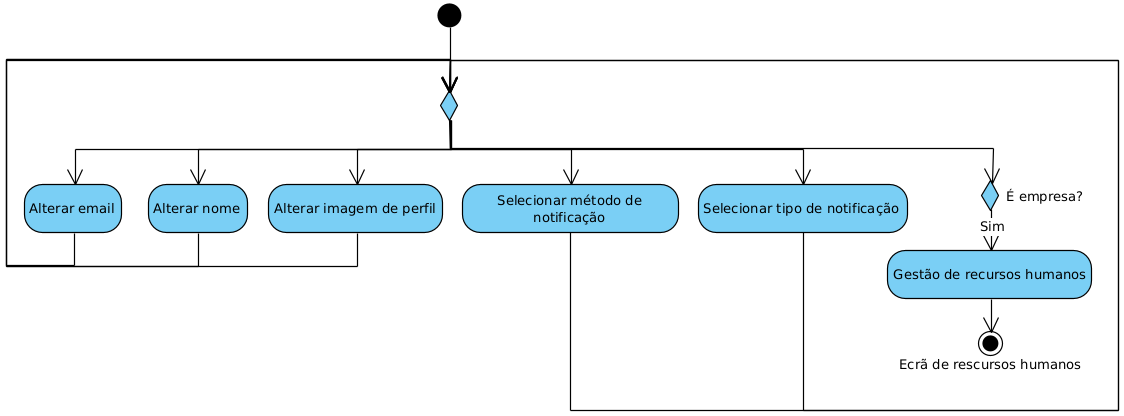
\includegraphics[width=\textwidth]{images/diagramas/atividades/diagrama_atividades_perfil.png}
    \caption{Diagrama de atividades de página de perfil}
    \label{fig:35}
\end{figure}

\newpage

\subsection{Diagrama de atividades página inicial do fórum}

Na página inicial do fórum o técnico poderá selecionar um dos tipos de pesquisa, escrita ou código QR, filtrar por tipo, ver as listagens de tópicos em destaque, mais recentes, por responder, os seus tópicos e criar um novo tópico. Estas listagens poderão ser filtradas por tipo e sobre as mesmas tem a possibilidade de selecionar um tópico o que o redirecionará para o ecrã de detalhes.

\begin{figure}[htb]
    \centering
    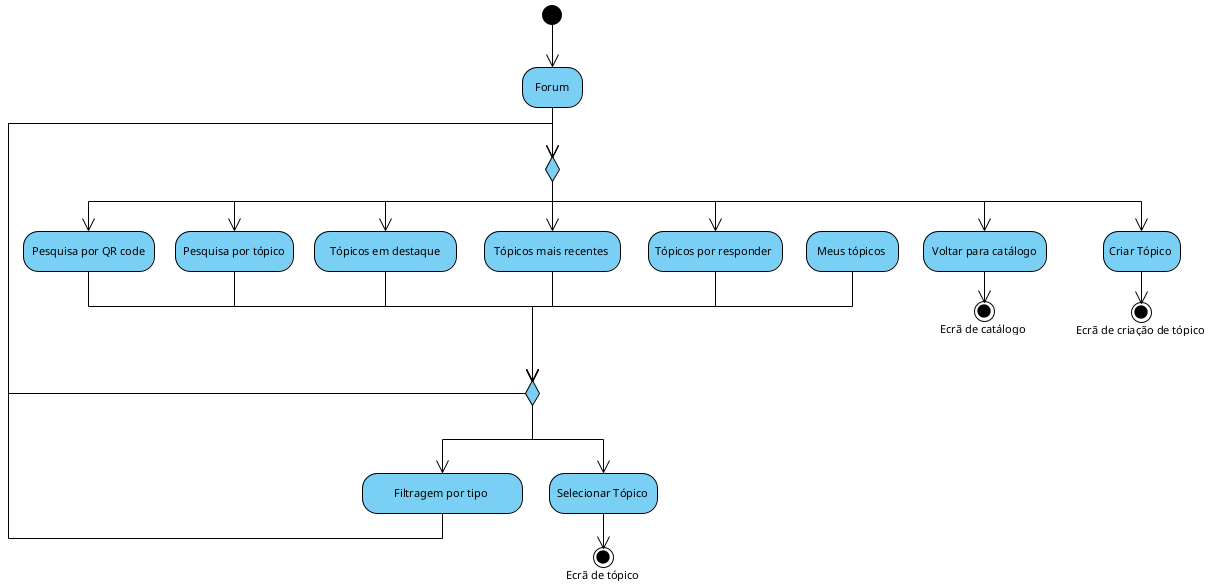
\includegraphics[width=\textwidth]{images/diagramas/atividades/diagrama_atividades_forum.png}
    \caption{Diagrama de atividades de página inicial do fórum}
    \label{fig:36}
\end{figure}

\newpage

\subsection{Diagrama de atividades página de criação de tópico}

Quando o técnico decide criar um tópico, obrigatoriamente tem de indicar o título, a descrição e o tipo do tópico. Por predefinição a visibilidade deste é pública, mas o técnico poderá alterar. Facultativamente o técnico poderá indicar o produto referente ao tópico, assim como anexar e remover imagens. A qualquer momento, o técnico poderá confirmar a criação do tópico, quando esta ação inicia, é realizada uma verificação do título e da descrição para concluir se estão preenchidos. Caso estes dados não estejam preenchidos é indicado ao técnico que as informações estão em falta, caso contrário este volta para o ecrã anterior.

\begin{figure}[htb]
    \centering
    \includegraphics[width=0.7\textwidth]{images/diagramas/atividades/diagrama_atividades_criar_tópico.png}
    \caption{Diagrama de atividades de página de criação de tópico}
    \label{fig:37}
\end{figure}

\newpage

\subsection{Diagrama de atividades página de detalhes do tópico}

Assim que o técnico seleciona um tópico, este poderá visualizar todos os comentários, apagar um caso seja seu, gostar do tópico e/ou de uma resposta, comentar e responder a um comentário. Caso o tópico seja do técnico, este poderá também alterar a visibilidade, marcar como concluído ou remover. A qualquer momento, o técnico tem como possibilidade retroceder para o ecrã anterior.

\begin{figure}[htb]
    \centering
    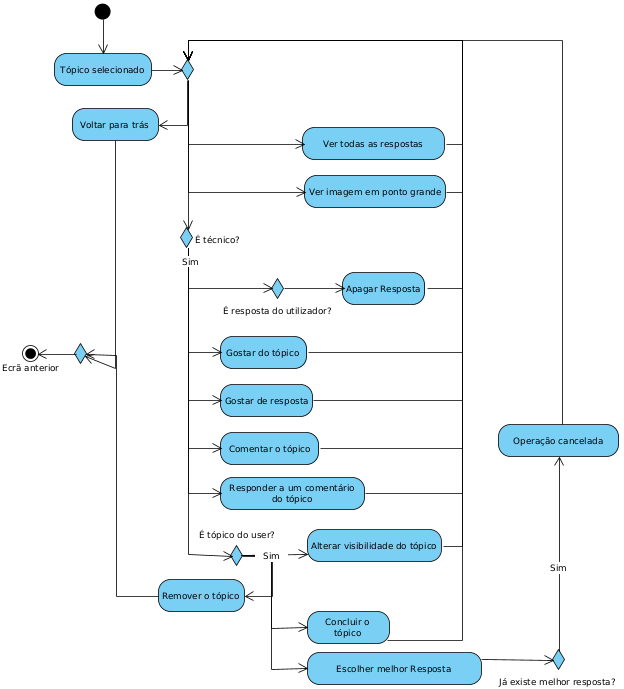
\includegraphics[width=0.9\textwidth]{images/diagramas/atividades/diagrama_atividades_detalhes_topico.png}
    \caption{Diagrama de atividades de página de detalhes do tópico}
    \label{fig:38}
\end{figure}

\newpage

\subsection{Diagrama de atividades páginas de autenticação}

Para realizar a ativação da conta do técnico, assim que este realiza o registo, confirmação da conta ou o login com uma conta que não se encontra ativa, este é encaminhado para o ecrã de ativação da conta. Neste ecrã poderá cancelar e indicar o código de ativação. Se o código estiver errado, o técnico deverá inserir-lo novamente. Por outro lado, se inserir um código correto a conta será validada e o técnico ficará autenticado. Também, em caso de necessidade, o proprietário da conta terá como opção pedir o envio de um novo código de ativação.

\begin{figure}[htb]
    \centering
    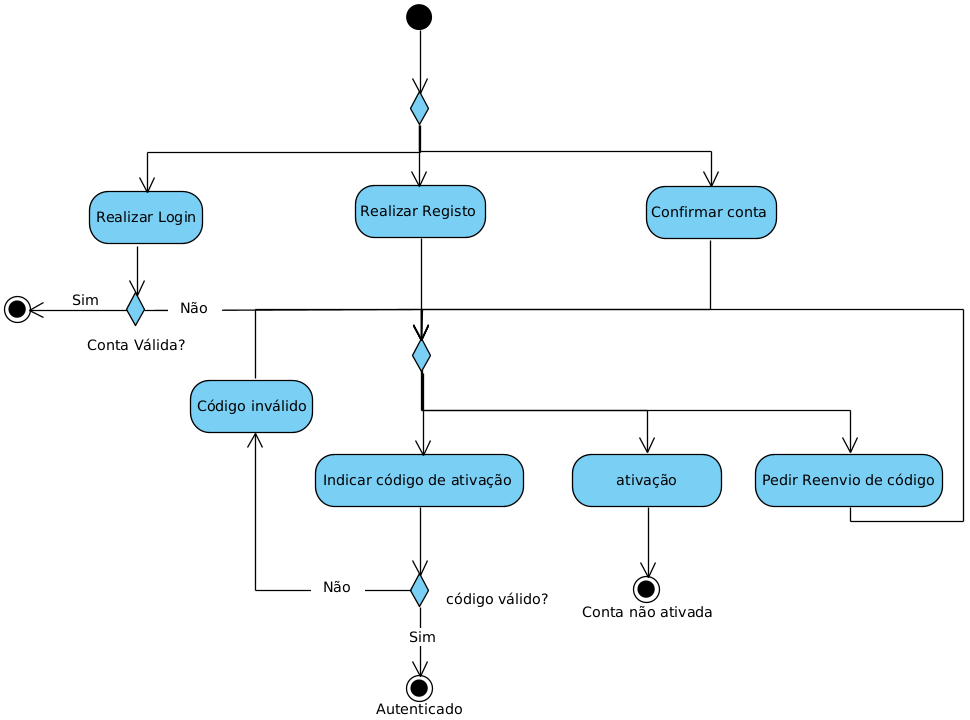
\includegraphics[width=0.8\textwidth]{images/diagramas/atividades/diagrama_atividades_autenticação.png}
    \caption{Diagrama de atividades de página de validação de conta}
    \label{fig:39}
\end{figure}

\newpage

% \subsection{Diagrama de atividades página de notificações}

% Sempre que o técnico recebe uma notificação, este poderá ver esta notificação no ecrã de notificações, 
% Este ecrã permite ao utilizador selecionar uma notificação sendo redirecionado para o tópico referente,
% caso esta esteja referente a um tópico, ou então poderá apagar a notificação.

% \begin{figure}[htb]
%     \centering
%     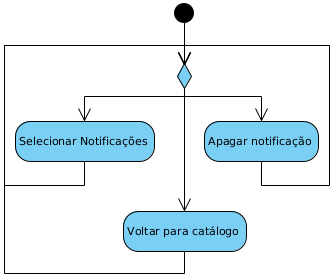
\includegraphics[width=0.5\textwidth]{images/diagramas/atividades/diagrama_atividades_noti.png}
%     \caption{Diagrama de atividades de página de notificações}
%     \label{fig:27}
% \end{figure}

% \subsection{Diagrama de atividades gestão de recursos humanos}

% Uma empresa poderá gerir as contas dos seus recursos humanos, para isso deverá se dirigir a este ecrã.
% Neste ecrã é possível registar um novo técnico sendo encaminhada para o ecrã de registo de técnico, 
% selecionar um técnico sendo encaminhada para o ecrã de perfil do técnico e poderá também pesquisar por 
% técnico.

% \begin{figure}[htb]
%     \centering
%     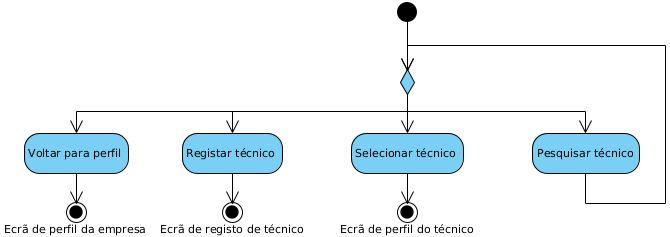
\includegraphics[width=\textwidth]{images/diagramas/atividades/diagrama_atividades_human_resources.png}
%     \caption{Diagrama de atividades de página de recursos humanos}
%     \label{fig:29}
% \end{figure}


% \subsection{Diagrama de atividades perfil de técnico}

% Sempre que uma empresa seleciona um técnico, esta é encaminhada para o ecrã de perfil de técnico. Neste 
% ecrã é possível impedir acesso à plataforma e remover a conta de técnico da plataforma.

% \begin{figure}[htb]
%     \centering
%     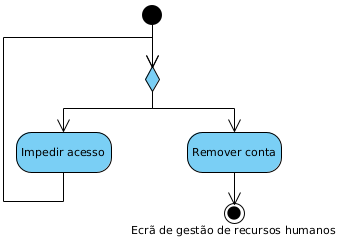
\includegraphics[width=0.5\textwidth]{images/diagramas/atividades/diagrama_atividades_prof_profile.png}
%     \caption{Diagrama de atividades de página de perfil de técnico}
%     \label{fig:30}
% \end{figure}

\newpage

\subsection{Diagrama de atividades registar técnico}

Assim que uma empresa inicia o registo de um técnico, esta é redirecionada para a página de registo do técnico. Nesta página, terá de indicar o nome, o \textit{email} e o tipo de técnico. Por fim será capaz de confirmar o registo da conta e automaticamente a empresa é movida para a página anterior.

\begin{figure}[htb]
    \centering
    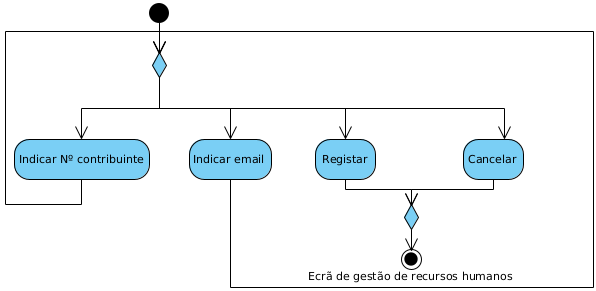
\includegraphics[width=0.8\textwidth]{images/diagramas/atividades/diagrama_atividades_add_professional.png}
    \caption{Diagrama de atividades de página de registar técnico}
    \label{fig:31}
\end{figure}

\subsection{Diagrama de atividades confirmar conta}

Quando uma conta de técnico é registada, um \textit{email} de confirmação é enviado para o técnico. Assim que este o recebe, deverá clicar em confirmar a conta. A partir desta ação, este move-se para a página de confirmação da conta. Nesta página, o técnico poderá alterar o seu \textit{email}, indicar o nome, a \textit{password} e a confirmação da \textit{password}.Todo o processo termina quando o botão de registar for pressionado.

\begin{figure}[htb]
    \centering
    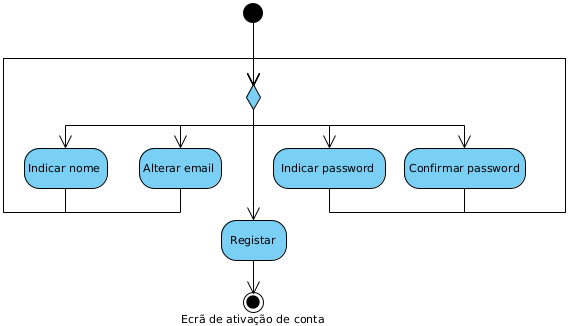
\includegraphics[width=0.8\textwidth]{images/diagramas/atividades/diagrama_atividades_prof_register.png}
    \caption{Diagrama de atividades de página de confirmar conta de técnico}
    \label{fig:31}
\end{figure}